\documentclass[12pt, a4paper]{article}

% --- PAKIETY JĘZYKOWE I KODOWANIE ---
\usepackage[utf8]{inputenc}
\usepackage[T1]{fontenc}
\usepackage[polish]{babel}
\usepackage{lmodern} % Nowocześniejsza czcionka

% --- GRAFIKA, KOLORY I RAMKI ---
\usepackage{graphicx}
\usepackage{float}
\usepackage{xcolor}
\usepackage{tcolorbox} % Ramki do "efektów specjalnych"
\usepackage{fontawesome5} % Ikony (np. symbol procesora, kropli wody)
\usepackage{fancybox}
\usepackage{bookmark}

% --- KONFIGURACJA KOLORÓW ---
\definecolor{arduino_teal}{RGB}{0, 151, 156}
\definecolor{code_bg}{RGB}{40, 44, 52} % Ciemne tło w stylu One Dark
\definecolor{soft_gray}{RGB}{245, 245, 245}

% --- KOD PROGRAMISTYCZNY (MINTED) ---
\usepackage{minted}
\setminted{
	style=monokai,       % Wyrazisty schemat kolorów (ciemny)
	bgcolor=code_bg,     % Ciemne tło dla kontrastu
	linenos=true,        % Numery linii
	frame=lines,         % Linie góra/dół
	framesep=10pt,
	fontsize=\footnotesize,
	breaklines=true,     % Zawijanie długich linii
	tabsize=2
}

% --- NAGŁÓWKI I STOPKI ---
\usepackage{fancyhdr}
\pagestyle{fancy}
\fancyhf{}
\fancyfoot[R]{\textbf{\thepage}}
\renewcommand{\headrulewidth}{0.4pt}
\fancyhead[L]{\textit{Projekt: Badanie wody}}

\usepackage{parskip}
\usepackage{titlesec}

\titleformat{\section}
{\large\bfseries\color{arduino_teal}}
{\thesection}{1em}{}


% --- METADANE ---
\title{
	\vspace{-2cm}
	
\includegraphics[width=3cm]{arduino_logo.png}\\ % Opcjonalne logo
	\Huge \textbf{Badanie przejrzystości wody}\\[8pt]
	\Large \textcolor{arduino_teal}{System monitorowania TDS z Arduino Uno}
}
\author{\textbf{Jakub Dostojewski} \\ Klasa 3F}
\date{\today}

\begin{document}
	
	\begin{titlepage}
		\maketitle
		\thispagestyle{empty}
		\vfill
		\begin{center}
			\begin{tcolorbox}[colback=arduino_teal!5,colframe=arduino_teal,title=Opis techniczny]
				Urządzenie wykorzystuje czujnik analogowy TDS oraz DHT11 do precyzyjnego pomiaru zanieczyszczenia cieczy z kompensacją temperaturową.
			\end{tcolorbox}
		\end{center}
	\end{titlepage}
	
	\setcounter{page}{2}
	\tableofcontents
	\newpage
	
	\section{Wstęp}
	\subsection{Spis sprzętu \faTools}
	\begin{itemize}
		\item[\faMicrochip] \textbf{Arduino Uno rev. 3} --- 1 szt.
		\item[\faTint] \textbf{Czujnik TDS} --- 1 szt.
		\item[\faThermometerHalf] \textbf{Czujnik DHT11} --- 1 szt.
		\item[\faTv] \textbf{Wyświetlacz LCD 16x2} --- 1 szt.
		\item[\textcolor{red}{\faCircle}]\textbf{Dioda LED (czerwona)} --- 1 szt.
		\item[\faWaveSquare]\textbf{Rezystory 220$\Omega$} --- 2 szt.
		\item[\faProjectDiagram] \textbf{Płytka stykowa i przewody}
	\end{itemize}
	
	\subsection{Podstawy teoretyczne \faBook}
	\begin{tcolorbox}[colback=blue!5, colframe=blue!50!black, title=Czym jest TDS?]
		TDS (\textit{Total Dissolved Solids}) mierzy całkowitą ilość substancji rozpuszczonych w wodzie. 
		Pomiar odbywa się poprzez badanie \textbf{przewodności elektrycznej}. 
		Wartość podawana jest w jednostkach \textbf{ppm} (\textit{parts per million}).
	\end{tcolorbox}
	
	\subsection{Wykorzystane oprogramowanie \faLaptopCode}
	\begin{tcolorbox}[colback=soft_gray, colframe=black, title=Środowisko programistyczne]
		\begin{itemize}
			\item Arduino IDE 2.3.8 dla systemu Arch Linux\texttrademark – tworzenie i wgrywanie programu do mikrokontrolera
			\item Fritzing 1.0.6 dla systemu Microsoft Windows 11 – wykonanie schematu połączeń na płytce stykowej
			\item KiCad 10.0 dla systemu Arch Linux\texttrademark – profesjonalny schemat elektryczny
			\item TeXstudio 4.9.3 dla systemu Arch Linux\texttrademark – przygotowanie dokumentacji projektu w \LaTeX
		\end{itemize}
	\end{tcolorbox}
	
	\newpage
	
	\section{Zasada działania systemu \faCogs}
	\begin{tcolorbox}[colback=arduino_teal!5,colframe=arduino_teal,title=Opis działania]
		Układ mierzy przewodność elektryczną cieczy za pomocą czujnika TDS. 
		Na podstawie odczytanego napięcia obliczana jest wartość ppm.
		
		Temperatura odczytywana z czujnika DHT11 służy do kompensacji błędu pomiarowego (jest to temperatura otoczenia - do obliczeń w stopniach Celsjusza, natomiast ta wyświetlana na ekranie LCD jest przeliczona na stopnie Kelvina).
		
		Wyniki są wyświetlane na ekranie LCD, a przekroczenie ustalonego progu 
		zanieczyszczenia powoduje zapalenie się diody LED.
	\end{tcolorbox}
	
	\section{Kod źródłowy programu \faCode}
	\begin{center}
		\small \textit{Implementacja w języku C++ z wykorzystaniem filtracji medianowej}
	\end{center}
	
	% Stylizowany blok kodu
	\begin{minted}{cpp}
// Libraries
#include <LiquidCrystal.h>
#include <dht.h>

// Constant variables and pins
#define TdsSensorPin A0
#define dhtPin 2
#define ledPin 3
#define VREF 5.0      // Reference voltage of ADC
#define SCOUNT 30     // Number of samples for median filter

int analogBuffer[SCOUNT];     // Buffer for raw TDS samples
int analogBufferTemp[SCOUNT]; // Temporary buffer for sorting
int analogBufferIndex = 0, copyIndex = 0, check;

float averageVoltage = 0, tdsValue = 0, Temperature, temperatureKelvin;

// Members of classes: lcd for LiquidCrystal (display) and DHT for dht class (sensor)
LiquidCrystal lcd(7, 8, 9, 10, 11, 12);
dht DHT;

// Setting serial port, lcd display and pins
void setup() { 
	lcd.begin(16, 2);
	pinMode(TdsSensorPin, INPUT);
	pinMode(ledPin, OUTPUT);
	pinMode(dhtPin, INPUT);
	Serial.begin(9600);
} 

void loop() { 
	// Reading temperature from DHT11 and calculating Kelvin scale
	static unsigned long analogSampleTimepoint = millis();
	check = DHT.read11(dhtPin);
	if(check == 0) Temperature = DHT.temperature;
	temperatureKelvin = Temperature + 273.15;
	
	// Sampling TDS sensor every 40ms and storing in circular buffer
	if (millis() - analogSampleTimepoint > 40U) {
		analogSampleTimepoint = millis();
		analogBuffer[analogBufferIndex] = analogRead(TdsSensorPin);
		analogBufferIndex++;
		if (analogBufferIndex == SCOUNT) analogBufferIndex = 0;
	}
	
	static unsigned long printTimepoint = millis();
	
	// Processing and displaying data every 800ms
	if (millis() - printTimepoint > 800U) {
		printTimepoint = millis();
		
		// Copying buffer for filtering (to keep original data intact)
		for (copyIndex = 0; copyIndex < SCOUNT; copyIndex++) analogBufferTemp[copyIndex] = analogBuffer[copyIndex];
		
		// Getting median voltage and converting to real voltage value
		averageVoltage = getMedianNum(analogBufferTemp, SCOUNT) * (float)VREF / 1024.0;
		
		// Temperature compensation (standard reference 25*C)
		float compensationCoefficient = 1.0 + 0.02 * (Temperature - 25.0);
		float compensationVoltage = averageVoltage / compensationCoefficient;
		
		// Converting voltage to TDS value (ppm) using polynomial equation
		tdsValue = (133.42 * pow(compensationVoltage, 3) - 255.86 * pow(compensationVoltage, 2) + 857.39 * compensationVoltage) * 0.5;
		
		// High TDS alarm - LED indicator
		if(tdsValue >= 300) digitalWrite(ledPin, HIGH);
		else digitalWrite(ledPin, LOW);
		
		// Refreshing LCD with TDS results and temperature in Kelvin
		lcd.clear();
		lcd.setCursor(0, 0);
		lcd.print("TDS: ");
		lcd.print(tdsValue, 0);
		lcd.print("ppm");
		
		lcd.setCursor(0, 1);
		lcd.print("T: ");
		lcd.print(temperatureKelvin, 0);
		lcd.print("K");
	}
}

// Median filter function: sorts the array and returns the middle value
int getMedianNum(int bArray[], int iFilterLen) {
	int bTab[iFilterLen];
	for (byte i = 0; i < iFilterLen; i++) bTab[i] = bArray[i];
	
	int i, j, bTemp;
	
	// Simple Bubble Sort algorithm
	for (j = 0; j < iFilterLen - 1; j++) {
		for (i = 0; i < iFilterLen - j - 1; i++) {
			if (bTab[i] > bTab[i + 1]) {
				bTemp = bTab[i];
				bTab[i] = bTab[i + 1];
				bTab[i + 1] = bTemp;
			}
		}
	}
	
	// Returning median based on odd/even length
	if ((iFilterLen & 1) > 0) bTemp = bTab[(iFilterLen - 1) / 2];
	else bTemp = (bTab[iFilterLen / 2] + bTab[iFilterLen / 2 - 1]) / 2;
	
	return bTemp;
}
	\end{minted}
	
	\newpage
	
	\section{Schematy \faDraftingCompass}
	\subsection{Schemat uproszczony (Fritzing)}
	\begin{figure}[H]
		\centering
		\shadowbox{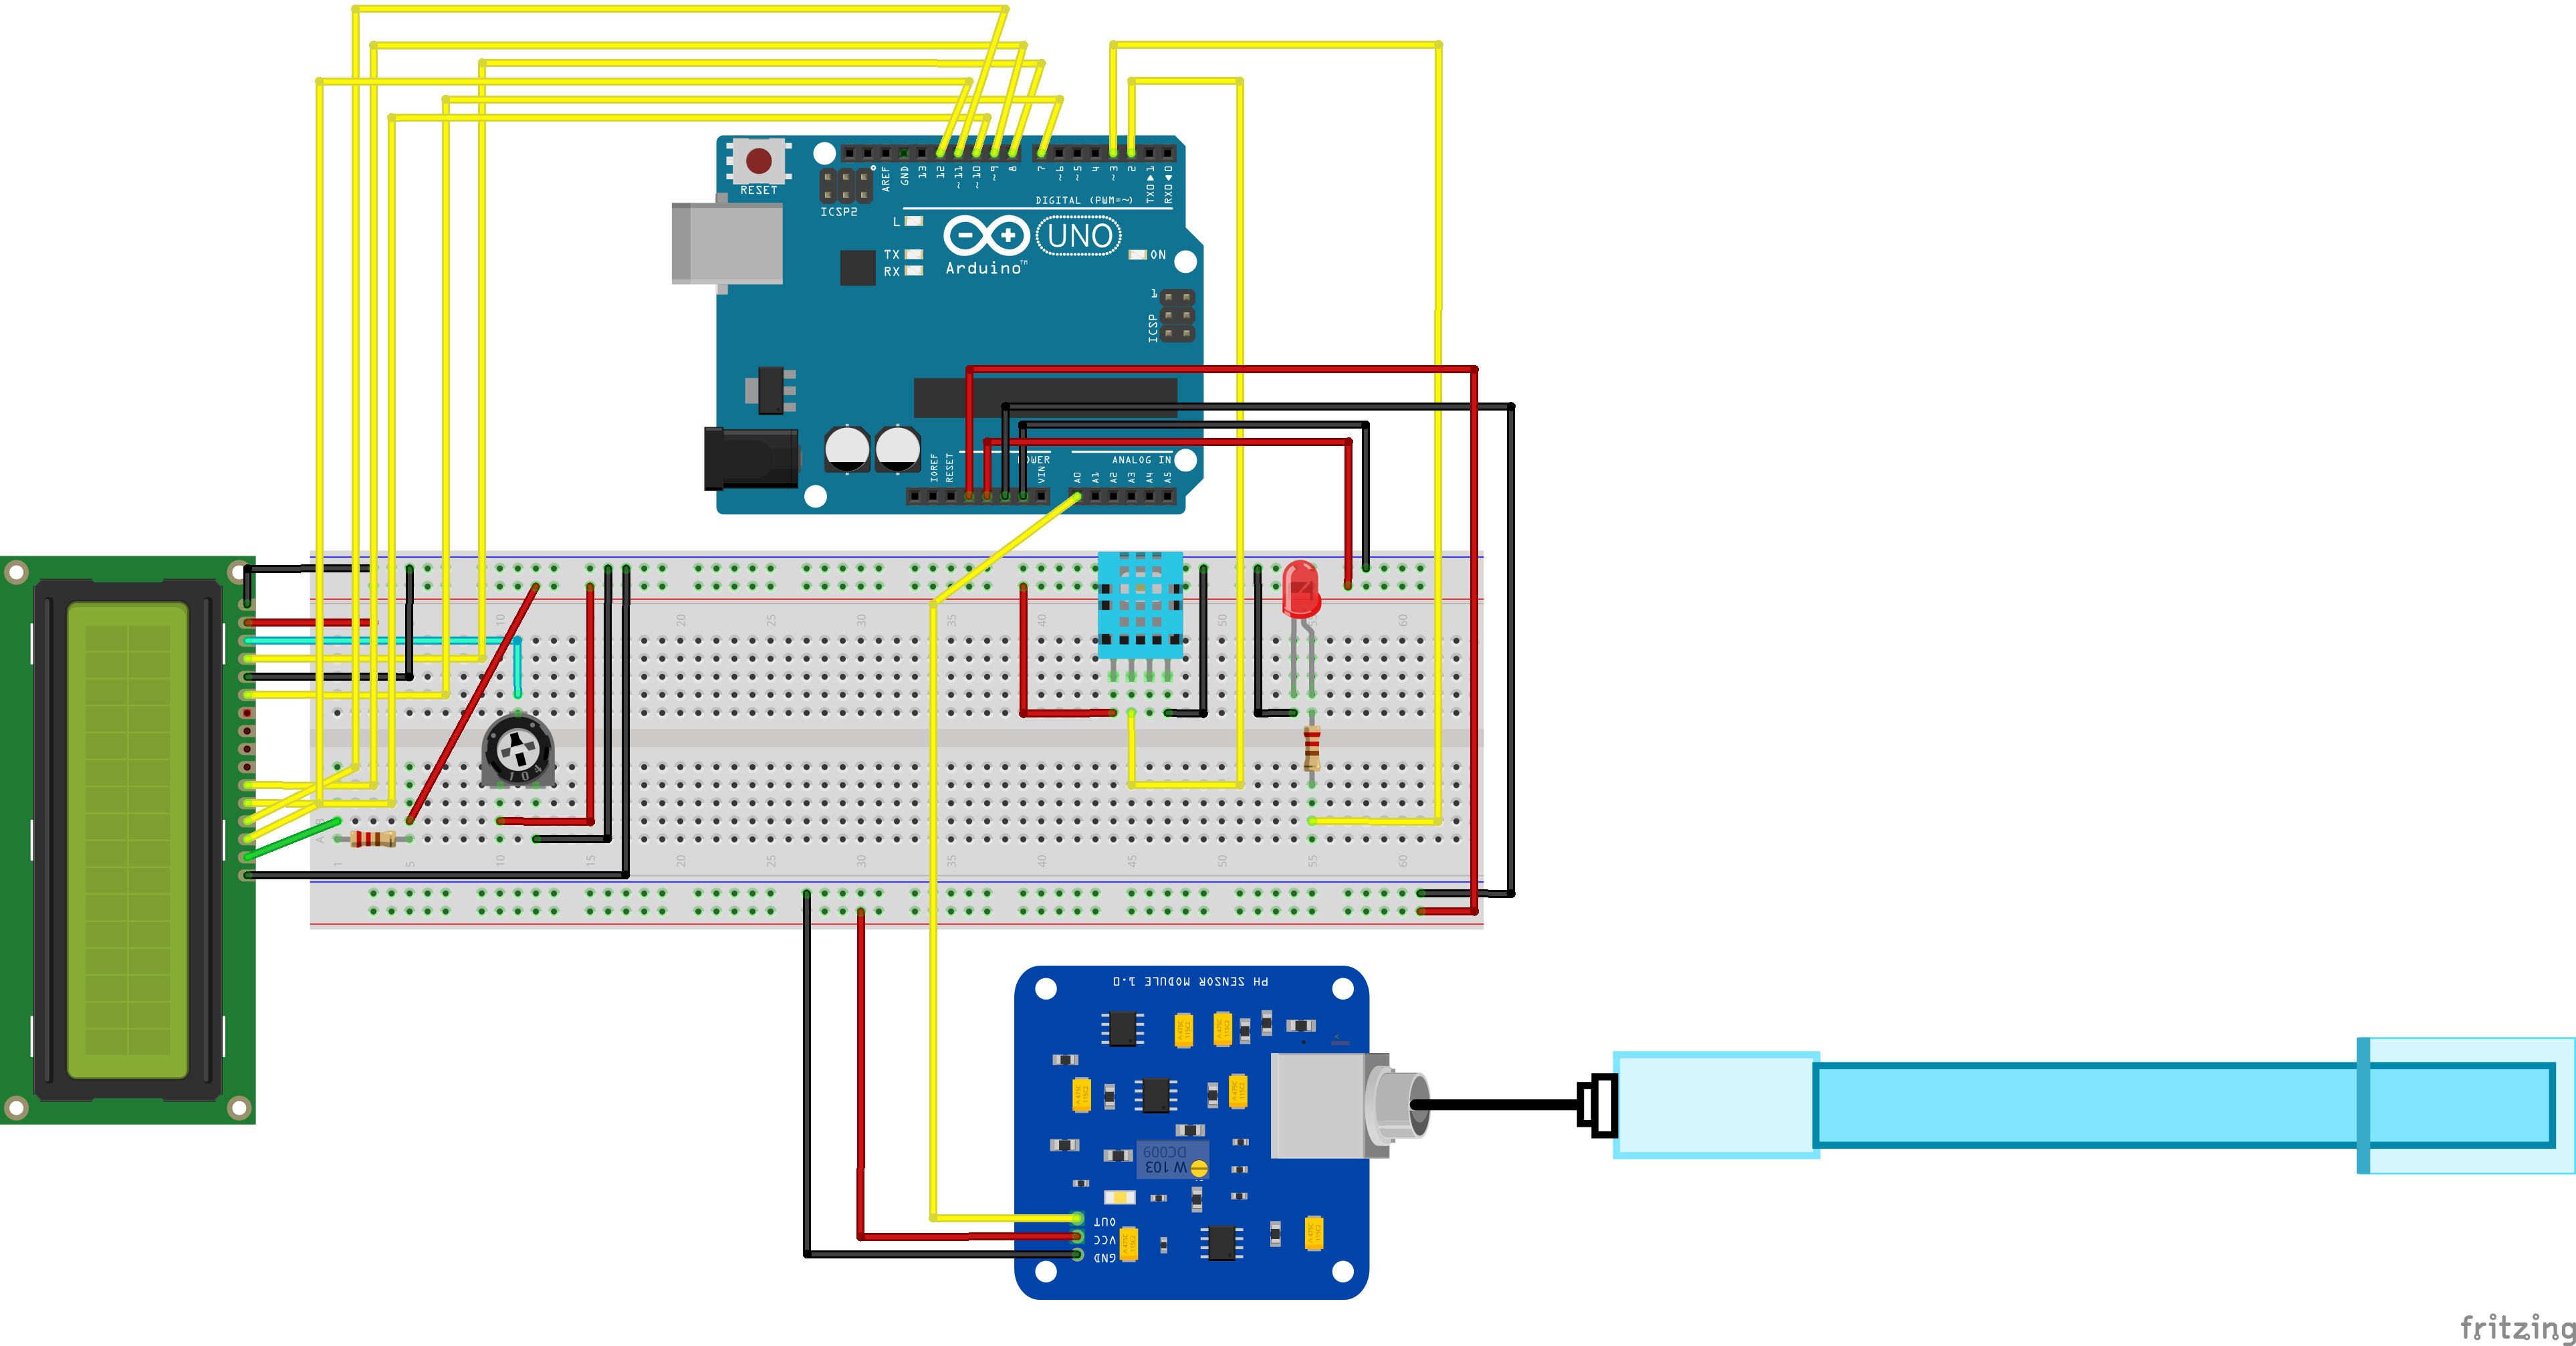
\includegraphics[width=0.85\textwidth]{arduino_lcd_tds_led_dht11.png}}
		\caption{Wizualizacja połączeń na płytce stykowej.}
	\end{figure}
		\subsection{Schemat rzeczywisty (KiCad)}
	\begin{figure}[H]
		\centering
		\shadowbox{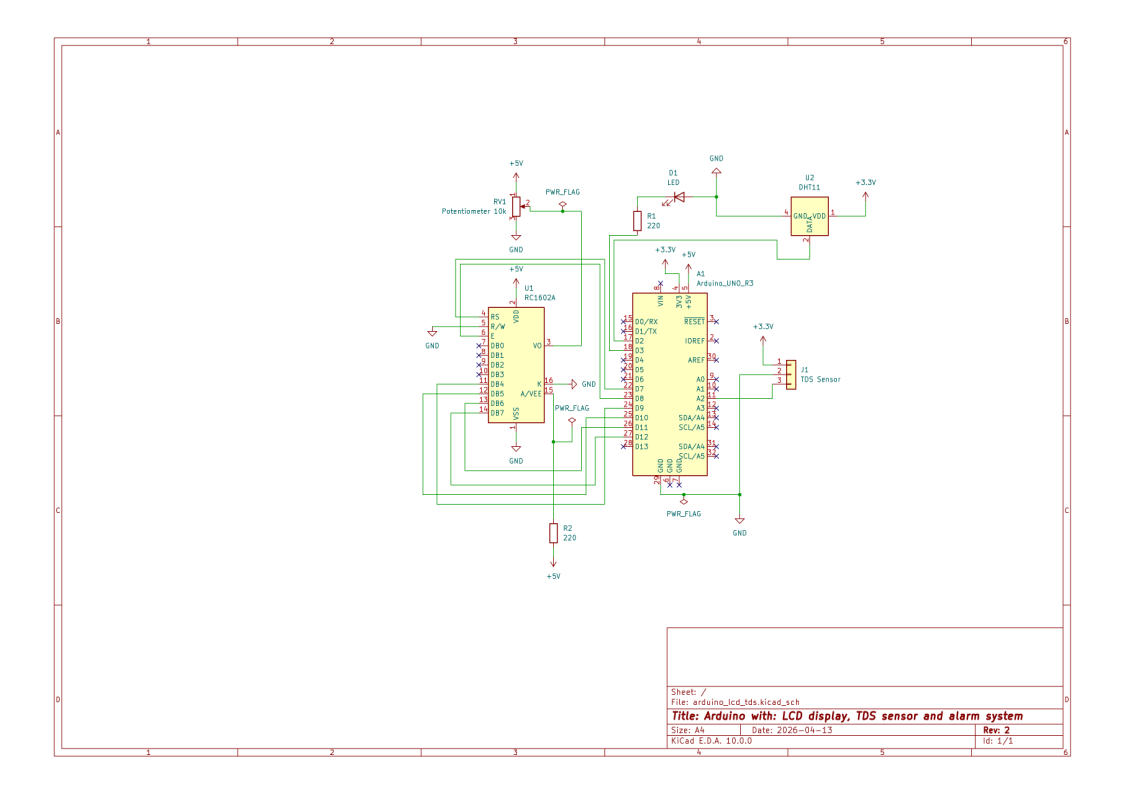
\includegraphics[width=0.85\textwidth]{schema.png}}
		\caption{Schemat elektryczny układu pomiarowego.}
	\end{figure}
	
	
\end{document}